\documentclass[runningheads]{llncs}
\usepackage[T1]{fontenc}
\usepackage{graphicx}
\usepackage{booktabs}
\newcommand{\corr}{(*)}
% N.B.: do not change anything above this line. If you require additional packages, please load them directly after this line.
% \usepackage{mwe} % optional

% Add extra packages here (after the line above)
\usepackage{amsmath,amssymb} 
\usepackage{cleveref}
\usepackage{algorithm}
\usepackage{algpseudocode} 
\usepackage{tikz}
 
\IfFileExists{xcolor.sty}{\usepackage{xcolor}}{\usepackage{color}}
\definecolor{dpgCritical}{rgb}{1.000,0.851,0.400}      % #ffd966
\definecolor{dpgPredBranch}{rgb}{0.714,0.843,0.659}    % #b6d7a8
\definecolor{dpgCompBranch}{rgb}{0.957,0.800,0.800}    % #f4cccc
\definecolor{dpgFocus}{rgb}{0.624,0.773,0.910}         % #9fc5e8
\definecolor{dpgContext}{rgb}{0.973,0.976,0.984}       % #f8f9fb
\definecolor{dpgTrueLeaf}{rgb}{0.576,0.769,0.490}      % #93c47d
\definecolor{dpgOtherLeaf}{rgb}{0.902,0.722,0.686}

\usepackage{longtable}

\usetikzlibrary{positioning,arrows.meta} 


\begin{document}

\title{%Decision Predicate Graphs for Faithful Local Explanations: Aligning Decision Structure and Outputs}
Decision Predicate Graphs for Structurally Faithful Local Explanations of Tree Ensembles Beyond Output Agreement}

\titlerunning{DPGs for Faithful Local Explanations}

% For double-blind submission (recommended for initial review), use:
% \author{Author information scrubbed for double-blind reviewing}
% \authorrunning{Anonymous Authors}

\author{Author information scrubbed for double-blind reviewing}
\authorrunning{Anonymous Authors}
\institute{}

\maketitle
\begin{abstract} %max 2000 chars
  Output-level agreement is an insufficient criterion for local explanations when the goal is to diagnose how a model reached a specific decision, since two explanations can match a prediction equally well while differing substantially in path-level faithfulness. We address this through Decision Predicate Graphs (DPGs), extending the original global construction to DPG-local, which builds each explanation as a sample-specific subgraph from the exact root-to-leaf paths executed by the ensemble. On top of this structure, a Semantic Graph View provides three diagnostics: an explanation confidence score, competitor exposure quantifying support for the strongest alternative class, and a critical node identifying where predicted and competing paths last overlap before diverging. Across 15 benchmark datasets, near-complete trace recovery (edge recall $\approx$ 0.99) confirms structural faithfulness, while edge precision and zero recombination serve as construction-consistency checks. DPG-local remains competitive on shared output-level metrics against TreeSHAP, ICE, LIME, and Anchors, while providing structurally grounded diagnostics that output-aligned methods cannot offer.
\keywords{Explainable AI \and Local explanations \and Tree ensembles \and Random forests \and Decision Predicate Graphs \and Structural faithfulness}
\end{abstract}

\section{Introduction}
Explainable AI methods are commonly distinguished by the scope of the explanation they provide. In the case of predictive modelling, global explanations aim to characterise the behaviour of a predictive model as a whole, whereas local explanations are designed to explain a single prediction of it or the model behaviour in the neighbourhood of a specific instance \cite{vilone2021notions}. 
Local
Explanations are especially important in decision-support settings because inspection, validation, contestability, and error analysis often arise at the micro level, that is, around an individual case rather than only at the macro level, that is, about the entire model behaviour \cite{nauta2023anecdotal}.
Many widely used local explanation methods are optimised for \emph{prediction-level} faithfulness and express explanations primarily through \emph{input features} or feature conditions. 
Local Interpretable Model-agnostic Explanations (LIME), for instance, explain a prediction by fitting an interpretable surrogate in the neighbourhood of the query point, whereas SHapley Additive exPlanations (SHAP) decompose the prediction into additive feature contributions relative to a reference baseline \cite{ribeiro2016why,lundberg2017unified}. 
Related methods, such as Individual Conditional Expectation (ICE) and Anchors, likewise describe local behaviour through feature-wise sensitivity profiles or sufficient rule conditions
\cite{goldstein2015ice,ribeiro2018anchors}.
In Fr\"amling's terminology, these methods predominantly characterise \emph{feature influence}, that is, effects defined with respect to a baseline or perturbation distribution, rather than the broader notion of feature importance \cite{framling2023importanceinfluence}.
Such a perspective is often useful, but it is not sufficient for the problem we target in this research study. 
When the objective is to inspect how a model arrived at a specific inference, diagnose failure modes, or compare competing class hypotheses, fidelity is understood as the degree to which an explanation accurately reflects its behaviour \cite{vilone2021notions}.
However, this is too weak a criterion when assessed only at the level of the final output. 
Different local explanations may exhibit similar prediction-level fidelity while differing substantially in whether they preserve the executed inferential path and expose the local decision structure that is diagnostically relevant.

In this research study, we investigate the hypothesis that \emph{Decision Predicate Graphs} (DPG) can serve as a faithful and informative basis for local explanations of tree-ensemble predictions, because they encode the model decision process directly at the level of standardised split predicates and their empirically observed transitions \cite{arrighi2024decision}. 
Accordingly, we represent each local explanation as a sample-specific sub-graph obtained by projecting the instance onto an obtained DPG. 
In this representation, nodes correspond to \emph{predicates} extracted from tree internal splits, that is, interpretable feature-value tests of the form $(x_j \leq \theta)$ (or $(x_j > \theta)$), where thresholds are mapped to a common vocabulary through rounding and consistent predicate formatting. 
Edges represent \emph{predicate transitions} activated along executed root-to-leaf paths, capturing the local ordering and co-occurrence of split conditions that lead to the predicted outcome. 
Our central thesis is that local graph explanations should be evaluated not only by agreement with a model's output, but also by how well they recover the executed decision structure and highlight where competing classes diverge. 
This matters because local explanations are often used to debug models, study errors, and compare alternative class hypotheses. 
In these settings, reproducing the predicted label is insufficient, and an explanation must reflect the decision route that is activated within a model for a specific input sample.
Accordingly, we position DPG-local as a complementary diagnostic layer for structural and contrastive analysis, rather than as a direct fidelity replacement for output-aligned methods such as TreeSHAP.

The reminder of the article is structured as follow.
Section \ref{sec:relWork} offers a presentation of related work within XAI, with a focus on local methods and their limitations.
Section \ref{sec:desMethods} introduced the design of a novel method based on a reformulation of the Decision Predicative Graph methods tailored to local explanations, along with the introduction a Semantic Graph View with class-contrastive, structure-aware descriptors. 
Section \ref{sec:experiments} defines the evaluation strategy for evaluating the novel method along with the baseline methods selected in the literature.
Section \ref{sec:results} presents the results of the empirical work, and findings are synthesised and discussed in section \ref{sec:discussion}.
Eventually, a synthesis of the contribution of the body of knowledge offered by this research is presented in section \ref{sec:conclusion}, proposing future areas of improvement.

\section{Related Work}\label{sec:relWork}
Local explanations for tabular predictors are often organised into feature attribution, local-surrogate, response-profile, and rule-based approaches \cite{molnar2019iml,adadi2018peeking} %,arrieta2020explainable}. 
This taxonomy reflects both the explanatory object returned by each method and the extent to which it is tied to an underlying model. It also mirrors how explanations are used in practice, where interpretability supports not only communication of predictions but also debugging, auditing, and disagreement analysis in high-impact settings \cite{arrieta2020explainable,doshi2017rigorous}.
Feature-attribution methods explain predictions through per-feature contribution scores. TreeSHAP is the most established model-direct local explainer for tree ensembles and provides additive feature attributions with strong alignment to the model output under the SHAP axioms \cite{lundberg2017unified,lundberg2018consistent}. TreeSHAP is therefore a necessary baseline for shared metrics such as output agreement, confidence and margin behaviour, and perturbation-based tests. However, it represents an explanation as a vector of feature contributions and does not return an explicit local decision structure. As a result, it does not directly support structural checks such as whether an explanation preserves executed predicate transitions, whether predicted and competing classes share a decision gate, or whether candidate paths arise from recombining fragments that never co-occurred in any executed trace.

Local surrogates and rule-based explainers provide explanations through simplified models or sufficient conditions. LIME fits an interpretable surrogate in the neighbourhood of an instance using perturbation sampling, and its coefficients are commonly interpreted as local feature influence \cite{ribeiro2016why}. Anchors produces high-precision local rules intended to preserve the prediction under perturbations and reports precision and coverage \cite{ribeiro2018anchors}. 
Beyond single-rule summaries, several methods represent local explanations as sets of rules extracted from tree ensembles. Building Explanations Through a Locally Accurate Rule EXtractor (BELLATREX) explains a Random Forest prediction using a small and diverse set of representative rules selected from the forest, aiming to increase coverage of alternative local rationales while keeping the explanation compact \cite{dedja2023bellatrex}. 
Related rule-extraction lines, such as RuleFit and rule ensembles, also rely on tree-derived rule features, typically to build an interpretable model or compact rule set that can be inspected locally \cite{friedman2008predictive}.
While these methods operate over interpretable predicates, they primarily return rule lists or surrogate rule models rather than a local graph object whose transitions and branching structure can be validated against executed traces.
In particular, BELLATREX is closer to DPG-local than LIME/ICE in that it is model-direct and tree-derived, but it still returns a selected rule set rather than an ordered predicate-transition graph. Therefore, it does not preserve the full transition ordering of executed paths as a first-class output, and it does not provide an explicit recombination diagnostic against executed transitions.
The same limitation applies to RuleFit/rule ensembles, which encode tree logic as rule features or compact rule lists, not as verifiable local path graphs.

Response-profile methods focus on what-if behaviour rather than reconstructing local reasoning. ICE plots vary a single feature while keeping others fixed and visualise the corresponding change in model output, revealing non-linear effects and heterogeneity across instances \cite{goldstein2015ice}. ICE is valuable as a sensitivity diagnostic, but it does not represent the route taken by a tree ensemble for a specific instance and does not encode explicit competition between predicted and alternative classes. We also include a tree-path baseline that follows executed forest paths and aggregates them into feature-level contributions \cite{palczewska2014interpreting}. This baseline is closer in spirit to our DPG-local perspective, but it reduces structure to a feature ranking: executed predicates are projected to per-feature scores, path transitions are not retained as graph edges, and predicted-versus-competitor branch competition is not represented explicitly.

%Our Semantic Graph View is motivated by two 
Recurring observations on local methods exists.
First, explanations are often contrastive, since users naturally ask why a model favored one outcome over plausible alternatives \cite{miller2019explanation}. Second, different explainers can disagree substantially for the same model and input, which affects how explanations are used for debugging and decision making \cite{krishna2022disagreement}. These observations motivate reporting competitor exposure and explicit predicted-versus-competitor comparisons, rather than only a single-class summary. Recent evaluation work further emphasizes that output-level fidelity alone is insufficient and that faithfulness should be assessed through complementary criteria \cite{nauta2023anecdotal,doshi2017rigorous}. 
%In line with this view, we evaluate all methods using shared metrics where applicable, and we complement them with structural measures that are meaningful only for DPG-local graphs.

Table~\ref{tab:positioning} summarizes the reviewed XAI methods, which will act as baselines in this research and allow to situate and situates our proposal. 
DPG-local explanations differ from attribution, surrogate, response-profile, and rule summaries by targeting a DPG-local graph whose nodes are split predicates and whose edges are the predicate transitions activated by the ensemble on the inspected sample \cite{arrighi2024decision}. This representation supports structure-dependent diagnostics, including competitor-path competition and critical decision gates, while remaining comparable to prior work on shared output-level metrics.
For \Cref{tab:positioning}, ``partial'' structural faithfulness ($\sim$) means that a method uses tree-derived predicates or path fragments but does not return a local graph with ordered predicate transitions that can be validated edge by edge against executed traces. Under this criterion, BELLATREX and RuleFit are ``partial'' because they return rule sets/models rather than transition graphs, and tree-path is ``partial'' because it follows executed paths but collapses them into feature rankings without preserving branch topology. ``Supported'' ($\checkmark$) requires all three properties: (i) explicit transition ordering, (ii) branch/topology preservation, and (iii) direct trace-level structural checks (edge recall/precision and recombination diagnostics).

\begin{table}[t]
\centering
\caption{Positioning of local explanation methods. Symbols indicate support ($\checkmark$), partial support ($\sim$), or not supported ($\times$). Access uses \texttt{d} for model-direct and \texttt{a} for model-agnostic. Faith.\ denotes structural faithfulness checks against executed traces, and Contrast denotes explicit predicted-versus-competitor diagnostics.}
\label{tab:positioning}
\small
\setlength{\tabcolsep}{6pt}
\begin{tabular}{l l c c c}
\hline
Method & Object & Access & Faith. & Contrast \\
\hline
TreeSHAP \cite{lundberg2018consistent} & feature attributions & \texttt{d} & $\times$ & $\sim$ \\
LIME \cite{ribeiro2016why} & local surrogate & \texttt{a} & $\times$ & $\sim$ \\
ICE \cite{goldstein2015ice} & response profile & \texttt{a} & $\times$ & $\times$ \\
Anchors \cite{ribeiro2018anchors} & rule conditions & \texttt{a} & $\times$ & $\sim$ \\
BELLATREX \cite{dedja2023bellatrex} & diverse rule set & \texttt{d} & $\sim$ & $\sim$ \\
RuleFit / rule ens. \cite{friedman2008predictive} & rule model / rule set & \texttt{d} & $\sim$ & $\sim$ \\
Tree-path \cite{palczewska2014interpreting} & path-based ranking & \texttt{d} & $\sim$ & $\times$ \\
\hline
DPG-local (ours) & DPG-local graph & \texttt{d} & $\checkmark$ & $\checkmark$ \\
\hline
\end{tabular}
\end{table}





\section{Design and methods}\label{sec:desMethods}
To enable DPG-based local explanations, we modify the graph construction used in the original DPG formulation and its extension \cite{arrighi2024decision,ceschin2025extending}. 
Instead of aggregating predicate transitions across the dataset, we build each local graph from the exact root-to-leaf paths executed by the ensemble for the target sample. Aggregated transitions can splice together fragments that never appeared on the same tree path, yielding plausible labels but invalid local routes and weaker separation between the predicted and competing classes. Our DPG-local construction avoids this issue and allows the resulting local graph to be verified directly against the model’s executed traces.
On the obtained DPG, we introduce a Semantic Graph View for structured local explanations. It reports (i) an \emph{explanation confidence score}, (ii) \emph{competitor exposure}, which quantifies how much support is assigned to the strongest alternative class, and (iii) a \emph{critical decision node}, defined as the last shared non-root predicate between the strongest predicted path and the strongest competitor path. These quantities are designed to go beyond aggregate benchmarking and to support disagreement-aware analysis and error diagnosis, in line with evidence that explanation disagreement is common in practice and requires explicit treatment \cite{krishna2022disagreement}. 
Moreover, by explicitly contrasting the predicted outcome with a competing alternative, this Semantic Graph View follows the broader view that explanations are often contrastive in nature \cite{miller2019explanation}. 


\begin{figure}[t]
\centering
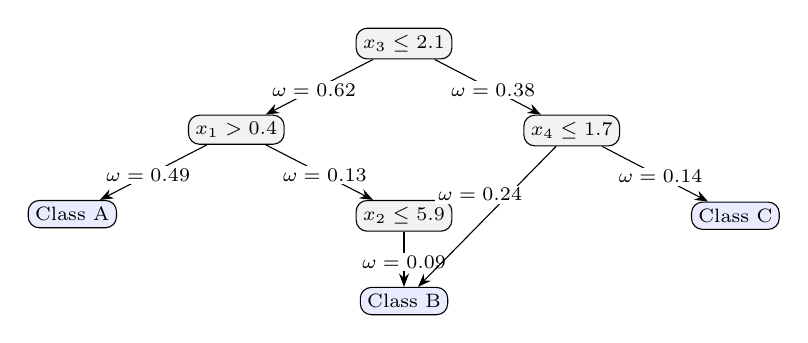
\begin{tikzpicture}[
  >=Stealth,
  node distance=7mm and 9mm,
  pred/.style={rectangle, rounded corners, draw=black, fill=gray!10, align=center, font=\scriptsize, inner sep=2.5pt},
  cls/.style={rectangle, rounded corners, draw=black, fill=blue!8, align=center, font=\scriptsize, inner sep=2.5pt},
  elab/.style={font=\scriptsize, fill=white, inner sep=1pt}
]
\node[pred] (p1) {$x_3 \le 2.1$};
\node[pred, below left=of p1] (p2) {$x_1 > 0.4$};
\node[pred, below right=of p1] (p3) {$x_4 \le 1.7$};
\node[pred, below right=of p2] (p4) {$x_2 \le 5.9$};
\node[cls, below left=of p2] (cA) {Class A};
\node[cls, below=of p4] (cB) {Class B};
\node[cls, below right=of p3] (cC) {Class C};

\draw[->] (p1) -- node[elab, pos=0.55] {$\omega=0.62$} (p2);
\draw[->] (p1) -- node[elab, pos=0.55] {$\omega=0.38$} (p3);
\draw[->] (p2) -- node[elab, pos=0.55] {$\omega=0.49$} (cA);
\draw[->] (p2) -- node[elab, pos=0.55] {$\omega=0.13$} (p4);
\draw[->] (p4) -- node[elab, pos=0.55] {$\omega=0.09$} (cB);
\draw[->] (p3) -- node[elab, pos=0.55, above, yshift=7pt] {$\omega=0.24$} (cB);
\draw[->] (p3) -- node[elab, pos=0.55] {$\omega=0.14$} (cC);
\end{tikzpicture}
\caption{Illustrative DPG-local graph for one sample. Rectangles are
standardized predicate nodes, rounded blue rectangles are class terminals, and edge labels are
normalized transition support. Dominant routes and competitor routes can be
inspected directly from edge support and branching structure.}
\label{fig:dpg-example}
\end{figure}

\subsection{DPG and the Local-Explanation Gap}
Decision Predicate Graphs (DPGs) were introduced as an interpretable graph representation for tree ensembles that can be visualised, but whose main role for explanation is enabling the extraction of graph metrics such as local reaching centrality, betweenness centrality, and community detection, where nodes are standardised split predicates and edges capture observed predicate transitions \cite{arrighi2024decision}. 
Its extension presented in \cite{ceschin2025extending} reinforced the value of this representation for model inspection. However, the original construction focuses on global explainability: transitions are aggregated across samples.
In DPG, each node denotes a standardised split predicate (for example, $x_j \le \theta$, where $x_j$ is the value of the $j$-th feature of sample $x$, $j$ is the feature index, and $\theta$ is the split threshold), and each directed edge denotes an observed transition between two predicates along tree traversals. Edge weights summarise how frequently that transition is observed in the ensemble, so the graph captures not only connectivity but also transition strength. This structure is useful for explainability because it keeps the decision process in an interpretable predicate language and makes dominant versus weak decision routes explicit, as illustrated in \Cref{fig:dpg-example}.


A limitation appears in how the original global DPG is constructed and queried. Since transitions are aggregated over many samples, traversing the global graph for a single instance can follow edges that are individually valid but were not jointly executed for that instance. 
In other words, local routes can be assembled by stitching transition fragments from different samples or different trees. 
This weakens local faithfulness when the explanation target is the exact executed decision process rather than only the final predicted label.
For local explanation, this creates a mismatch with the problem raised in \Cref{tab:positioning}: many methods can preserve output labels but do not preserve the executed decision structure for the inspected sample \cite{nauta2023anecdotal,krishna2022disagreement}. When transitions are aggregated globally, a local traversal may combine edge fragments that never co-occurred in any single tree execution for that sample. We refer to this as \emph{recombination}.
Our objective is to preserve DPG as a data structure while replacing its local construction rule: local graphs must be built from exact sample-specific execution traces, not from global transition statistics. The details of these DPG improvements, formalized as DPG-local construction, are presented in \Cref{sec:dpg-construction}.

\subsection{DPG-local Construction}
\label{sec:dpg-construction}
Let $\mathcal{F}=\{T_b\}_{b=1}^B$ be a trained tree ensemble with $B$
baselearners, where $T_b$ denotes the $b$-th baselearner. For a sample $x$, let
$\pi_b(x)=[p^{(b)}_1,\dots,p^{(b)}_{L_b}]$ be the executed root-to-leaf predicate sequence in baselearner $T_b$, where $L_b$ is its path length. Predicates are standardized with a deterministic map $\phi(\cdot)$ (feature naming plus threshold rounding).
The key difference from the original DPG is the construction scope. The original version aggregates transitions across many samples to build a global graph, whereas the DPG-local version builds $G_x$ using only the transitions executed for the inspected sample $x$. Therefore, the local graph contains sample-specific realised transitions, not globally valid but potentially non-co-occurring transition fragments.
The computational profile also differs. If a global DPG is built from $N$ samples, the aggregation stage is approximately $O(NB\bar{L})$, where $\bar{L}$ is the average executed path length; local explanation then requires an additional query/traversal step on the global graph. In the DPG-local version (our proposal), constructing one local graph is $O(BL_x)$ for sample $x$ (or
$O(B\bar{L})$ on average, because only sample-specific executed traces are processed. Over all $N$ samples, the total asymptotic cost remains on the same order, but the DPG-local pipeline shifts computation to per-sample local construction and removes dependence on a separate global-graph traversal stage.
The decision predicate graph is $G_x=(V_x,E_x,\omega_x)$:
\begin{itemize}
  \item $V_x$: set of standardised predicate nodes reached for sample $x$;
  \item $E_x$: set of directed transitions between consecutive predicates in executed paths;
  \item $\omega_x(e)$: normalized support of edge $e$, computed as its
        frequency across the $B$ baselearners.
\end{itemize}
Hence, every edge in $G_x$ is backed by at least one executed trace for $x$. From this construction, we obtain graph descriptors that directly support model explainability at the local level. Node support indicates how often each predicate node appears in executed paths for $x$, which helps separate stable conditions from incidental ones. Edge support indicates how often each transition is observed, making dominant and weak local routes explicit. Class-terminal support reports how much total path support ends in each class node, so predicted-versus-competitor evidence can be inspected directly. Branching concentration indicates whether support after a predicate is focused on one successor or dispersed across alternatives, clarifying whether the local decision is decisive or contested. Together, these descriptors summarise how the
ensemble \emph{actually traversed} predicates for $x$. 
The formal semantic and faithfulness metrics built from these quantities are defined in \Cref{sec:semantic-layer,sec:structural-faithfulness}.
The full construction procedure is reported in \Cref{alg:exec-trace-dpg}.
The per-sample construction cost is linear in executed path length,
$O(\sum_{b=1}^{B}L_b)$, with memory $O(|V_x|+|E_x|)$. Because the main design claim of DPG-local is to avoid stitching transitions
that were never jointly executed for the inspected sample, we track
recombination directly after construction. With
$\Gamma_x=E_x^{edge}\setminus T_x^{edge}$, the recombination rate is
\[
\mathrm{RecombinationRate}_x=\frac{|\Gamma_x|}{|E_x^{edge}|+\varepsilon}.
\]
This metric is central in our evaluation: lower values indicate fewer
non-executed transition fragments in the local explanation graph.


\begin{algorithm}[ht!]
\caption{DPG-local construction}
\label{alg:exec-trace-dpg}
\begin{algorithmic}[1]
\Require sample $x$, tree ensemble $\mathcal{F}=\{T_b\}_{b=1}^B$, standardization map $\phi$
\Ensure local graph $G_x=(V_x,E_x,\omega_x)$
\State $V_x \gets \emptyset$, $E_x \gets \emptyset$
\State $c_e \gets$ empty map from edges to counts
\For{$b=1$ to $B$}
  \State $\pi_b(x) \gets$ executed root-to-leaf predicate sequence in $T_b$
  \State $\hat{\pi}_b(x) \gets [\phi(p)\ \text{for}\ p\in\pi_b(x)]$
  \State add all predicates in $\hat{\pi}_b(x)$ to $V_x$
  \For{each consecutive pair $(u,v)$ in $\hat{\pi}_b(x)$}
    \State add $(u,v)$ to $E_x$
    \State $c_e[(u,v)] \gets c_e[(u,v)] + 1$
  \EndFor
\EndFor
\For{each edge $e\in E_x$}
  \State $\omega_x(e) \gets c_e[e]/B$
\EndFor
\State \Return $G_x=(V_x,E_x,\omega_x)$
\end{algorithmic}
\end{algorithm}



\subsection{Semantic Graph View} \label{sec:semantic-layer}

The DPG-local construction in Section~3.2 gives a trace-faithful local graph,
but diagnosis requires compact quantities that can be compared across samples
and datasets. We therefore derive a small set of metrics that target the three
needs stated in Section~1: separation between predicted and competing classes,
assessment of whether evidence is concentrated or diffuse, and agreement between
the explanation and the ensemble decision. The confidence score aggregates these
signals under structural coverage, so high confidence is reported only when both
semantic support and trace recovery are strong.
From $G_x$, we extract weighted explanation paths
\[
\mathcal{P}_x=\{(p,w_x(p),y(p))\},
\]
where $p$ is a local path, $w_x(p)\ge 0$ is its support, and $y(p)$ is its
class endpoint. We normalise supports as
\[
\tilde{w}_x(p)=\frac{w_x(p)}{\sum_{q\in\mathcal{P}_x} w_x(q)+\varepsilon},
\]
with $\varepsilon=10^{-12}$ for numerical stability. Class support is then obtained by summing normalised path support over all paths ending in class $y$; we denote this quantity by $S_x(y)$. The explanation class $\hat{y}^{exp}_x$ is the class with the largest support, and the strongest competitor $y_x^{(2)}$ is the non-predicted class with the highest remaining support. 
Using these quantities, the Semantic Graph View reports connected diagnostics rather than a single score. The margin $M_x=S_x(\hat{y}^{exp}_x)-S_x(y_x^{(2)})$ measures separation between predicted and competitor classes. Path purity is the support assigned to the predicted class, $\mathrm{PathPurity}_x=S_x(\hat{y}^{exp}_x)$, and competitor exposure is its complement, $\mathrm{CompetitorExposure}_x=1-\mathrm{PathPurity}_x$. To capture whether evidence is concentrated on a few dominant predicted-class paths, we use top-$K$ concentration $C_x^{(K)}$ (with $K=3$ in our
experiments).
We also compute explanation-to-ensemble vote agreement. Let $V_x(y)$ be the number of base-learners voting for class $y$ on sample $x$; then $A_x=V_x(\hat{y}^{exp}_x)/B$ quantifies how aligned the explanation-predicted class is with the ensemble vote. Finally, structural coverage is $G_x^{cov}=(R_x^{node}+R_x^{edge})/2$, and we combine the three semantic components with coverage as
\[
\mathrm{Conf}_x=G_x^{cov}\cdot\frac{M_x+C_x^{(K)}+A_x}{3}.
\]
The combination is scale-consistent: since path supports are normalised, $S_x(y)\in[0,1]$ and therefore $M_x\in[0,1]$ (predicted-class support minus strongest-competitor support); by definition $C_x^{(K)}\in[0,1]$,
$A_x\in[0,1]$, and $G_x^{cov}\in[0,1]$. Hence $\mathrm{Conf}_x\in[0,1]$.
We use an unweighted mean for $(M_x,C_x^{(K)},A_x)$ to avoid dataset-specific tuning and to keep the score interpretable as a balanced semantic summary.
Coverage is applied multiplicatively as a reliability gate: even strong semantic Signals should be down-weighted when trace recovery is weak. This confidence is not a probability-calibration measure but rather a compact summary of structural coverage, class separation, evidence concentration, and agreement with the
ensemble decision.
Table~\ref{tab:semantic-metrics} summarises the semantic-view metrics and their explainability use.

\begin{table}[t]
\centering
\small
\caption{Semantic Graph View metrics and explainability use.}
\label{tab:semantic-metrics}
\setlength{\tabcolsep}{5pt}
\begin{tabular}{p{3.4cm} p{8.1cm}}
\toprule
Metric & Explainability use \\
\midrule
Class support & Quantifies evidence assigned to each class from local paths. \\
\addlinespace[1pt]
Predicted/competitor class & Identifies the explained outcome and the strongest alternative for contrastive analysis. \\
\addlinespace[1pt]
Margin & Measures separation between predicted and competitor classes. \\
\addlinespace[1pt]
Path purity & Indicates how much support remains on the predicted class. \\
\addlinespace[1pt]
Competitor exposure & Indicates how much support shifts toward alternative classes. \\
\addlinespace[1pt]
Top-$K$ concentration & Shows whether evidence is concentrated in a few dominant paths. \\
\addlinespace[1pt]
Vote agreement & Checks alignment between explanation class and ensemble voting behavior. \\
\addlinespace[1pt]
Structural coverage & Summarizes node/edge recovery of executed traces. \\
\addlinespace[1pt]
Explanation confidence & Provides a single structure-aware summary of local explanation quality. \\
\bottomrule
\end{tabular}
\end{table}

\subsection{Critical Node and Structural Faithfulness}
\label{sec:structural-faithfulness}

We use the strongest predicted-class path and the strongest competitor path to
localize where the explanation route diverges. Let $p_x^\ast$ denote the
highest-weight path for $\hat{y}^{exp}_x$ and $q_x^\ast$ the highest-weight path
for $y_x^{(2)}$. We compare these two ordered node sequences through their
longest common prefix. If the common prefix ends at the root (or immediately
after it), we do not report a non-root critical node. Otherwise, the last shared
non-root predicate is the critical node $c_x$, and its prefix position is the
critical depth $d_x$. After that split, we compare post-split support toward the
predicted and competitor successors; branch contrast is
$\Delta_x^{crit}=|B_x(s_x^{pred})-B_x(s_x^{comp})|$, where $B_x(\cdot)$ is
normalized branch support after the critical split. A visual example is shown
in \Cref{fig:critical-node-example}.
In practice, this improves local explainability because:
%\begin{itemize}
  i)it identifies the precise decision point where predicted and competitor explanations separate;
  ii) it enables contrastive reasoning (why the predicted class instead of the strongest alternative);
  iii) it localises sensitivity to specific predicates, supporting debugging and error diagnosis;
  iv) it supports targeted what-if analysis around the split where divergence occurs;
  v) It makes disagreement cases easier to interpret by characterising whether divergence is early, late, sharp, or weak.
%\end{itemize}

We then evaluate structural faithfulness against exact executed traces for the same sample $x$. Let $(T_x^{node},T_x^{edge})$ be trace node/edge sets and $(E_x^{node},E_x^{edge})$ the explanation node/edge sets. Node recall and node precision measure how much of the executed predicate set is recovered and how much of the recovered predicate set is valid. Edge recall and edge precision measure the same properties for predicate transitions. Concretely, each recall term is intersection-over-trace-size, and each precision term is intersection-over-explanation-size (with $\varepsilon=10^{-12}$ smoothing in denominators).
These metrics are complemented by the recombination rate (defined in
Section~3.2), which directly tests whether non-executed transition fragments appear in the local explanation graph.

\begin{figure}[h]
\centering
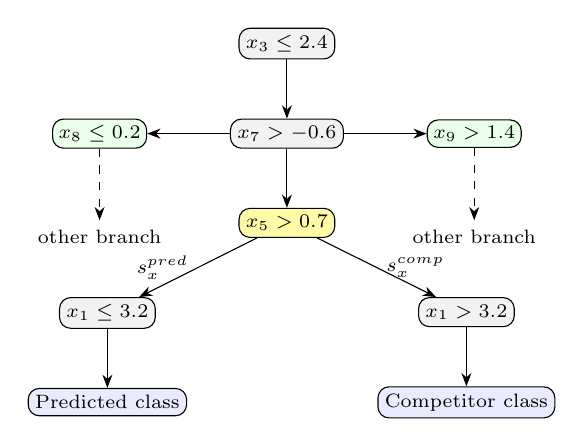
\begin{tikzpicture}[
  >=Stealth,
  node distance=7.5mm and 10.5mm,
  pred/.style={rectangle, rounded corners, draw=black, fill=gray!10, align=center, font=\scriptsize, inner sep=2.5pt},
  crit/.style={rectangle, rounded corners, draw=black, fill=yellow!35, align=center, font=\scriptsize, inner sep=2.5pt},
  cls/.style={rectangle, rounded corners, draw=black, fill=blue!8, align=center, font=\scriptsize, inner sep=2.5pt},
  side/.style={rectangle, rounded corners, draw=black, fill=green!8, align=center, font=\scriptsize, inner sep=2.2pt}
]
\node[pred] (p1) {$x_3 \le 2.4$};
\node[pred, below=of p1] (p2) {$x_7 > -0.6$};
\node[crit, below=of p2] (c) {$x_5 > 0.7$};

\node[pred, below left=of c] (pp1) {$x_1 \le 3.2$};
\node[cls, below=of pp1] (yp) {Predicted class};

\node[pred, below right=of c] (pc1) {$x_1 > 3.2$};
\node[cls, below=of pc1] (yc) {Competitor class};

\node[side, left=of p2] (s1) {$x_8 \le 0.2$};
\node[side, right=of p2] (s2) {$x_9 > 1.4$};

\draw[->] (p1) -- (p2);
\draw[->] (p2) -- (c);
\draw[->] (p2) -- (s1);
\draw[->] (p2) -- (s2);
\draw[->] (c) -- node[font=\scriptsize, left] {$s_x^{pred}$} (pp1);
\draw[->] (c) -- node[font=\scriptsize, right] {$s_x^{comp}$} (pc1);
\draw[->] (pp1) -- (yp);
\draw[->] (pc1) -- (yc);
\draw[dashed,->] (s1) -- ++(0,-1.1) node[below,font=\scriptsize] {other branch};
\draw[dashed,->] (s2) -- ++(0,-1.1) node[below,font=\scriptsize] {other branch};
\end{tikzpicture}
\caption{Critical-node example with a more complex local structure. The two strongest explanation paths share a longer prefix
\;$x_3 \le 2.4$ $\rightarrow$ $x_7 > -0.6$ $\rightarrow$
\textcolor{black}{critical node} and then diverge toward predicted and competitor successors. Further side branches highlight the local graph can contain alternatives that are not part of the two strongest paths.}
\label{fig:critical-node-example}
\end{figure}


\section{Experimental Setup}\label{sec:experiments}
\subsection{Datasets and Models}

We evaluate on a curated set of 15 numeric tabular classification datasets:
\texttt{banknote-authentication}, \texttt{breast\_cancer}, \texttt{diabetes},
\texttt{digits}, \texttt{ionosphere}, \texttt{iris}, \texttt{isolet},
\texttt{madelon}, \texttt{phoneme}, \texttt{qsar-biodeg}, \texttt{segment},
\texttt{spambase}, \texttt{vehicle}, \texttt{wdbc}, and \texttt{wine}.
These datasets cover binary and multiclass tasks with very different feature counts and levels of predicate reuse, which is important for evaluating whether local explanation structure remains faithful on both simple and harder ensemble decision boundaries.

\begin{table}[h!]
  \centering
  \small
  \caption{Dataset and model summary used. `Avg. RF Perf.' is the average Random Forest predictive performance across the selected configurations and seeds.}
  \label{tab:datasets-models-summary}
  \begin{tabular}{lcccc}
    \toprule
    Dataset & \#Classes & \#Features & \#Samples & Avg. RF Perf. \\
    \midrule
    banknote-authentication & 2 & 4 & 1372 & 0.963 \\
    breast\_cancer & 2 & 30 & 569 & 0.950 \\
    diabetes & 2 & 8 & 768 & 0.726 \\
    digits & 10 & 64 & 1797 & 0.848 \\
    ionosphere & 2 & 34 & 351 & 0.939 \\
    iris & 3 & 4 & 150 & 0.944 \\
    isolet & 26 & 617 & 7797 & 0.714 \\
    madelon & 2 & 500 & 2600 & 0.626 \\
    phoneme & 2 & 5 & 5404 & 0.818 \\
    qsar-biodeg & 2 & 41 & 1055 & 0.816 \\
    segment & 7 & 19 & 2310 & 0.850 \\
    spambase & 2 & 57 & 4601 & 0.906 \\
    vehicle & 4 & 18 & 846 & 0.695 \\
    wdbc & 2 & 30 & 569 & 0.956 \\
    wine & 3 & 13 & 178 & 0.987 \\
    \bottomrule
  \end{tabular}
\end{table}

For every dataset we train random forest classifiers with the same search space
used by the local-explanation pipeline:
$n_{\mathrm{estimators}} \in \{10,20\}$, $\mathrm{max\_depth}=4$,
$\mathrm{perc\_var} \in \{10^{-4},10^{-5}\}$,
and $\mathrm{decimal\_threshold}=6$.
Here, $\mathrm{perc\_var}$ is the minimum path-frequency ratio used to keep
predicate transitions in the DPG construction pipeline, and
$\mathrm{decimal\_threshold}$ is the number of decimal digits used to round split thresholds when predicates are standardized.
Each configuration is repeated with random seeds $27$ and $42$.
The reported DPG-local results correspond to the DPG-local construction only.
Within this search space, the best DPG-local configuration for each dataset is selected by ranking runs according to local match rate that means  $\mathrm{local\_matches\_model\_rate}$, the fraction of evaluated samples where the explanation class equals the model-predicted class, edge precision, node precision,
recombination rate, and explanation confidence.

\subsection{Compared Methods and Metrics}
The main comparison includes DPG-local, DPG-global, and five baselines: TreeSHAP, LIME, ICE, Anchors, and a tree-path baseline that aggregates the class-probability changes observed along the model's executed tree paths.
This mix intentionally covers both model-direct explanation families and a local surrogate baseline. TreeSHAP, the tree-path baseline, and the anchor rules are all evaluated on the trained random forest itself rather than on an auxiliary surrogate model, while LIME provides the local-surrogate reference point.
For the baseline methods, we use the same random forest grid as above. Baseline hyperparameters follow the implementation defaults used in our reproducibility pipeline: TreeSHAP uses a background set of 200 training instances; LIME uses 20 explanation features and 1000 perturbed samples; ICE uses 21 grid points; and Anchors uses a precision target of $0.95$, a maximum rule length of 4, and at most 12 candidate conditions per expansion step. For each dataset and method, we retain the best configuration produced by this grid search.
Across methods, we report only metrics that are meaningfully comparable across different explanation families. We use \emph{fidelity} as the fraction of samples for which the explained class matches the model prediction, and \emph{local accuracy} as the fraction of samples for which the explained class matches the ground-truth label; both quantities follow standard
output-level-oriented evaluation practice in XAI
\cite{vilone2021notions,nauta2023anecdotal,doshi2017rigorous}. We also report a \emph{margin} score, defined as the difference between the top explained class score and the strongest competitor score, to capture class separation in a contrastive spirit \cite{miller2019explanation}. Finally, we report \emph{sufficiency} and \emph{comprehensiveness} by, respectively, keeping only the features selected by the explanation, or removing them and reevaluating the original model, as recommended by recent evaluation surveys \cite{nauta2023anecdotal}.
The semantic-faithfulness protocol is controlled to avoid giving DPG-local a larger feature budget than the baselines. For each sample, the baseline methods are allocated the same number of selected features as the corresponding DPG-local explanation. Sufficiency is computed by replacing all other features with the training-set reference vector, while comprehensiveness removes the selected features and leaves the remaining input unchanged. We report both the resulting target-class and the probability drop with respect to the unperturbed prediction.

\subsubsection{DPG-local-Specific Metrics}
Beyond shared metrics, only DPG-local is evaluated on the path-level
and graph-level semantics because these quantities rely on an explicit local decision graph. Planned metrics include 
i) node and edge recall/precision with respect to the executed trace,
ii) recombination rate,
iii) explanation confidence,
iv) critical-node metrics, including split depth and branch contrast,
v) disagreement-aware cohort summaries,
vi)critical-branch intervention metrics. 
The cohort analysis groups each sample according to the relationship between the true label, the model prediction, and the explanation prediction, which lets us separate model-correct, model-wrong, recovery, and disagreement cases instead of collapsing them into a single mean. The critical-branch analysis is applied only to DPG-local samples with a non-root critical node. For those samples, we intervene on the predicates immediately after the critical split and measure whether the model probability shifts toward the competitor branch.

\subsection{Reporting and Statistical Analysis}

We report results at the dataset level and aggregate them across datasets only
after per-dataset selection of the best configuration for each method. This
avoids letting large datasets dominate the comparison and follows the intended
use of local explanation methods as per-instance diagnostics.
For the shared metrics, we summarise mean performance across the 15 datasets, report mean-rank tables, and use paired non-parametric tests on the dataset-level scores. Specifically, we use the Friedman test to assess whether there is a global difference across methods and paired Wilcoxon signed-rank tests to compare DPG-local against each baseline. Structural metrics, cohort summaries, and critical-branch analyses are reported separately because they are DPG-local-specific and do not have a direct analogue for the
attribution or rule-based baselines.

\section{Results and discussion}\label{sec:results}
\subsection{Baseline Comparison on Shared Metrics}
The shared quantitative results in \Cref{fig:per-dataset-results} should be interpreted as a comparison of optimisation targets, not as a single winner-takes-all ranking. 
The fidelity and local-accuracy panels show the expected dominance of TreeSHAP, Tree-path, and Anchors, because these baselines are explicitly designed to preserve the model output prediction. In contrast, ICE and LIME are model-agnostic perturbation methods, and DPG-local is optimised for structural faithfulness, such as a surrogate representation, so lower fidelity/local-accuracy values relative to output-aligned tree baselines are expected. The margin panel adds complementary information. Anchors remains strong on fidelity but close to zero on margin because it returns a sufficient rule for the predicted class without a graded competitor-score decomposition, whereas DPG-local often dominates ICE and LIME by explicitly modelling predicted-versus-competitor path support in the local graph.
%The statistical tests support this reading. 
For all three shared metrics, the Friedman test rejects the null hypothesis of equal method performance across datasets ($p < 10^{-6}$ in all cases). 
Paired Wilcoxon tests show that DPG-local is significantly below TreeSHAP and  tree-path  on fidelity ($p=0.0015$, $p=0.0015$) and local accuracy ($p=0.0012$, $p=0.0079$).
However, DPG-local is not significantly different from TreeSHAP in margin ($p=0.454$), significantly exceeding tree-path ($p<10^{-4}$), ICE ($p=0.0020$), LIME ($p<10^{-4}$), and Anchors ($p<10^{-4}$).

\begin{figure}[ht!]
  \centering
  
\includegraphics[width=\textwidth,height=1.2\textheight,keepaspectratio]{per_dataset_shared_metrics_heatmap.pdf}
  \caption{Per-dataset shared quantitative metrics visualised as heatmaps. Rows are datasets and columns are methods (including both DPG variants: DPG-local and DPG-global); darker cells indicate higher values.}
  \label{fig:per-dataset-results}
\end{figure}

 For margin specifically, Friedman gives $\chi^2(5)=61.47$, $p=6.04\times 10^{-12}$, and paired Wilcoxon against TreeSHAP gives $W=46$, $p=0.454$ (DPG-local higher on 10/15 datasets, lower on 5/15), while DPG-local is higher on all 15 datasets versus tree-path, LIME, and Anchors. The main quantitative result is therefore not that DPG-local dominates all baselines on raw output agreement, but that it remains competitive on the shared metrics while providing substantially stronger separation between the predicted class and its competitor. Compared with tree-path in particular, DPG-local keeps predicate-transition topology and explicit competitor branching as the explanatory object, rather than collapsing executed paths to feature rankings. The controlled internal ablation between DPG-global (aggregated transitions) and DPG-local supports this interpretation. Across the 15 datasets in \Cref{fig:per-dataset-results}, DPG-local improves mean fidelity from $0.88$ to $0.90$, mean local accuracy from $0.79$ to $0.80$, and mean margin from $0.63$ to $0.73$, with dataset-level wins of 8/15, 8/15, and 11/15, respectively. These gains also complement the structural view: when local explanations are required to remain faithful to the executed decision process, DPG-local is the safer choice than DPG-global. The structural metrics in \Cref{tab:dpg-structural} are consistent with the same trend: DPG-local preserves executed transitions with near-complete recovery (edge recall near $1.00$), while edge precision and zero recombination are consistent with the trace-restricted construction and therefore acts as a sanity check, and DPG-local avoids recombination artefacts that are intrinsic to global cross-instance
aggregation.
In this sense, DPG-local should be interpreted as complementary to TreeSHAP and tree-path: it adds a structure-aware diagnostic view (branch topology, competitor exposure, and critical nodes) rather than targeting the same optimisation objective as pure output-fidelity explainers.

\subsection{Semantic Faithfulness}
This subsection focuses on DPG-local, LIME, and ICE because they are directly comparable under the same perturbation-based, matched feature-budget protocol. Here, the comprehensiveness drop denotes the decrease in the predicted-class probability after removing the features selected by the explanation; higher values indicate that the selected subset captures features on which the model strongly relies. Under this subgroup protocol, DPG-local reaches a mean sufficiency probability of $0.54$ and a mean comprehensiveness drop of $0.13$, close to LIME ($0.55$ and $0.17$) and above ICE in comprehensiveness
($0.07$), as per table \ref{tab:semantic-faithfulness}.



\subsection{Structural Faithfulness, Disagreement, and Misclassification}

Structural metrics are the dimensions in which DPG-local construction
provides its main advantage. Since there is no directly comparable graph-based baseline in our setting, this subsection reports a DPG local-centred structural evaluation across datasets. Across all evaluated datasets, DPG-local explanations contain on average $17.30$ active paths and $57.50$ active nodes per sample, while preserving the executed model structure almost exactly: mean edge precision is $1.00$, mean edge recall is $1.00$, and mean recombination is $0.00$ (\Cref{tab:dpg-structural}). Under DPG-local construction, edge precision and recombination are expected near-deterministic consistency checks (only executed edges are inserted), so the key empirical structural result is the near-complete edge recall ($\approx 0.99$), which confirms that the constructed local graph retains almost all executed transitions in practice.

\begin{table}[t]
\centering
\small
\caption{DPG-local-specific structural and semantic diagnostics for
DPG-local. The first row reports overall averages across the 15 datasets; the remaining rows summarise agreement and cohort regimes. Higher is better for confidence, support margin, and path purity; lower is better for competitor exposure and recombination. Edge precision/recombination are treated as construction-consistency checks for DPG-local, while edge recall and cohort/disagreement shifts are the main empirical diagnostics.}
\label{tab:dpg-structural}
\begin{tabular}{lcccccc}
\toprule
Group & Conf. & Margin & Purity & Comp. Exp. & Edge Prec. & Recomb. \\
\midrule
Overall & 0.69 & 0.73 & -- & -- & 1.00 & 0.00 \\
Agree & 0.70 & 0.75 & -- & -- & -- & 0.00 \\
Disagree & 0.48 & 0.23 & -- & -- & -- & 0.00 \\
MC-EC & 0.71 & -- & 0.87 & 0.13 & 1.00 & 0.00 \\
MW-EM & 0.63 & -- & 0.77 & 0.24 & 1.00 & 0.00 \\
\bottomrule
\end{tabular}
\end{table}

The average explanation confidence is $0.69$. This should not be read as
``low'' in isolation: it is an average over both easy and hard datasets. In
practice, the hardest datasets reduce this mean substantially, especially
\texttt{isolet} ($0.42$), \texttt{digits} ($0.49$), \texttt{vehicle}
($0.62$), and \texttt{madelon} ($0.63$), where class competition and local ambiguity are stronger. By contrast, cleaner regimes such as
\texttt{ionosphere} ($0.82$) and \texttt{banknote-authentication} ($0.81$) show high confidence.

The cohort analysis shows that explanation structure changes systematically with agreement and error type. The dominant cohort is the model-correct, explanation-correct group (MC-EC), whose mean per-dataset rate is $0.79$. For this cohort, DPG-local explanations are also the cleanest: mean explanation confidence is $0.71$, mean path purity is $0.87$, and competitor exposure is only $0.13$ (\Cref{tab:dpg-structural}). By contrast, model-wrong explanations that follow the model error (MW-EM) remain relatively confident, with mean explanation confidence $0.63$ and path purity $0.77$, showing that a structurally coherent explanation can still support the wrong class when the ensemble itself is wrong.

The disagreement split is even more informative. When the explanation agrees with the model, the mean explanation confidence is $0.70$, the mean support margin is $0.75$, and the mean model-vote agreement is $0.84$. When the explanation disagrees with the model, these values drop to $0.48$, $0.23$, and $0.38$, respectively, even though trace coverage remains essentially perfect in both groups. The effect sizes are large: for DPG-local, the difference between disagreement and agreement cases has Cohen's $d=-1.97$ for explanation confidence, $d=-1.86$ for support margin, and $d=-2.97$ for model-vote agreement. At the same time, disagreement cases show a strong increase in competitor exposure ($0.61$ versus $0.18$, $d=2.18$).
This pattern supports the intended interpretation of the semantic metrics: disagreement is not random noise, but a measurable redistribution of support from the predicted class toward competing branches.

The critical-branch intervention analysis is stricter still because it only
applies when the predicted and competitor explanations share a non-root prefix.
Under this criterion, valid DPG-local critical-node interventions are
concentrated in a small subset of datasets. The clearest case is
\texttt{vehicle}, where eight DPG-local samples admit a non-root critical
node and the intervention flips toward the competitor branch in $37.50\%$ of
those cases. This does not contradict the near-zero global value in
\Cref{tab:semantic-faithfulness}: Table~4 reports a pooled rate over all
evaluated samples, most of which do not satisfy the valid-intervention
criterion, whereas the \texttt{vehicle} figure is a conditional rate computed
only on the eight valid \texttt{vehicle} cases. This is a meaningful result because it links the semantic notion
of a critical split to an observable change in model behaviour.


\begin{figure}[bt!]
\centering

\includegraphics[width=0.82\linewidth,trim={0 8.2cm 0 0},clip]{vehicle_56_execution_trace_aggregate.pdf}
\vspace{1mm} \\
{\tiny
\textbf{Node legend:}
\textcolor{dpgCritical}{$\blacksquare$} critical node\,\,
\textcolor{dpgPredBranch}{$\blacksquare$} predicted branch\,\,
\textcolor{dpgCompBranch}{$\blacksquare$} competitor branch\,\,
%\textcolor{dpgFocus}{$\blacksquare$} focused path\,\,
%\textcolor{dpgContext}{$\blacksquare$} context\,\,
%\textcolor{dpgTrueLeaf}{$\blacktriangle$} true-class leaf\,\,
%\textcolor{dpgOtherLeaf}{$\blacktriangle$} other-class leaf
}
\caption{DPG-local graph for \texttt{vehicle} sample 56 (final
Phase C analysis. The yellow node is the critical node. From this node, the red edge marks the predicted-class successor and the green edge marks the competitor successor. Blue-toned edges represent the remaining local context; thicker edges indicate higher support in the local subgraph.}
\label{fig:phase-cases}
\end{figure}


\subsection{Case Study}
The qualitative analysis uses local-subgraph that preserves readability while retaining enough context to inspect critical nodes, successor branches, and alternative class endpoints. \Cref{fig:phase-cases} reports one DPG-local example, \texttt{vehicle} sample $56$.
In this DPG-local structure, the \texttt{MAX.LENGTH\_ASPECT\_RATIO} which is $>-0.231807$  is the critical node (yellow). The two highlighted successors from that node lead to different outcomes: the red branch moves toward class $1$ (model prediction), whereas the green branch moves toward class $2$ (competitor/true class). Their close support, reflected by the small support margin ($0.04$), indicates a locally ambiguous decision in which a small structural shift after the critical split is sufficient to favour the competitor branch. This makes the sample a recovery/disagreement case and illustrates the diagnostic role of the critical node: it isolates the specific local gate where predicted-versus-competitor evidence diverges.

\subsection{Discussion} \label{sec:discussion}
The results support a clear contribution of DPG for local explanation in tree ensembles, as Table~\ref{tab:dpg-metrics-properties} shows. First, DPG preserves executed decision structure at the trace level, which is reflected by near-perfect edge recovery and negligible recombination in the structural evaluation. This indicates that the explanation graph remains aligned with what the model actually executed, rather than assembling plausible but non-executed transitions.
Second, DPG adds semantic diagnostics that are difficult to obtain from attribution vectors or single-rule summaries alone. The disagreement analysis shows consistent shifts in confidence, support margin, and competitor exposure, which makes the prediction/explanation mismatch interpretable rather than opaque.
The case-study evidence reinforces this point: critical-node analysis can localise where support diverges between predicted and competing classes and can therefore support error diagnosis.
Third, DPG remains practically competitive on shared metrics while providing a different explanatory object: a local decision graph with explicit branch competition. This combination is the main empirical advantage of the proposal: output-aware behaviour with structure-aware diagnostics.
One limitation is that DPG is specialised to tree ensembles and requires graph-based interpretation, so its benefits are strongest when structural diagnostics are part of the analysis objective.

\begin{table}[ht!]
\centering
\small
\caption{DPG properties advancing faithful local explanation state of the art.}
\label{tab:dpg-metrics-properties}
\begin{tabular}{p{3.3cm} p{8.5cm}}
\toprule
DPG property & Contribution to faithful local explanation \\
\midrule
Trace faithfulness & Preserves executed transitions as a verifiable local graph (edge precision/recall; recombination), beyond attribution/rule summaries. \\
Class contrast & Makes predicted-versus-competitor support explicit (confidence, margin, exposure), not only feature influence. \\
Critical-node & Identifies and tests the exact local split where competing class support diverges (critical node/intervention). \\
Diagnostic cohorts & Links explanation behaviour to agreement and misclassification cohorts (agree/disagree; MC-EC, MW-EM). \\
\bottomrule
\end{tabular}
\end{table}


\section{Conclusion}\label{sec:conclusion}
This research introduced an execution-trace formulation of Decision Predicate Graphs for local explanation in tree ensembles, together with semantic diagnostics based on explanation confidence, support margin, competitor exposure, and critical-node analysis. 
In detail, the contributions offered by this research are: 
\begin{itemize}
  \item we reformulated DPG by constructing each explanation as a DPG-local graph extracted from the exact root-to-leaf paths activated by a tree ensemble on the inspected sample, rather than from aggregated predicate-transition statistics.
  \item we distinguished DPG-local from tree-path summaries that also use executed paths: tree-path collapses evidence to feature-level rankings, whereas DPG-local preserves predicate-transition topology, branch competition, and critical decision gates as first-class local objects.
  \item we introduced a Semantic Graph View that summarizes each DPG-local subgraph with class-contrastive, structure-aware descriptors, including an explanation confidence score, competitor exposure from the strongest alternative paths, and a critical decision node.
  \item We evaluated the method on 15 numeric tabular datasets against TreeSHAP, LIME, ICE, Anchors, and a tree-path baseline using shared metrics (output agreement with the model, confidence and margin behavior, explanation size, and runtime) together with DPG-specific structural faithfulness metrics (predicate and transition recovery, and recombination rate).
\end{itemize}
In synthesis, the major contribution is a local explanation object that preserves executed decision structure while remaining interpretable, as supported by experimental findings.
Across 15 tabular datasets, execution-trace DPG achieved near-perfect structural faithfulness (edge precision $1.00$, edge recall $0.99$) with zero recombination, while remaining competitive on shared output-level metrics. The disagreement and case-study analyses further showed that DPG can localize where predicted and competitor support diverge, enabling more informative error diagnosis than output agreement alone.

%TODO: add a couple of lines on future work, and how this study can be extended


\bibliographystyle{plain}
\bibliography{bibliography}

\end{document}
